\subsection{Similarity and Congruence}


\textit{Prove theorems, justify steps, and solve problems involving \textbf{similarity} and \textbf{congruence}.}

\vspace{.5cm}



\subsubsection[similarity]{Similarity} 

Geometric similarity is a relation between two objects. Objects that have the same \textbf{shape} are said to be similar.

\paragraph*{triangle similarity} 

Triangles are similar if:all their angles are equal and corresponding sides are in the same ratio. There are three ways to find if two triangles are similar: 

AA, SAS and SSS:

\begin{description}
    \item[AA] AA stands for "angle, angle" and means that the triangles have two of their angles equal.
    \item[SAS] SAS stands for "side, angle, side" and means that we have two triangles where the ratio between two sides is the same as the ratio between another two sides and we we also know the included angles are equal. 
    \item[SSS] SSS stands for "side, side, side" and means that we have two triangles with all three pairs of corresponding sides in the same ratio. 
\end{description}

\subsubsection*{Similar Triangle Theorems}


The following are several properties of similar triangles. 

\paragraph*{Side-splitter Theorem}
This theorem is about lines that split a triangle into proportional side lengths.
\begin{figure}[h!]
    \centering
    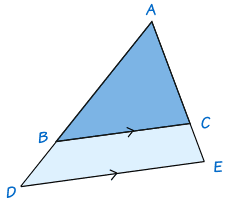
\includegraphics[width=2cm]{./public/images/side-splitter-theorem}
    \caption[side-splitter]{$BC \parallel DE \implies \frac{AB}{BD} = \frac{AC}{CE}$}
\end{figure}

\paragraph*{Angle Bisector Theorem}
This theorem is about proportional sides and angle bisectors.
\begin{figure}[h!]
    \centering
    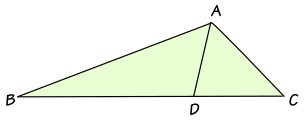
\includegraphics[width=3cm]{./public/images/angle-bisector-theorem}
    \caption[side-splitter]{$\overline{AD}  bisects \angle BAC \implies \frac{AB}{BD} = \frac{AC}{DC}$}
\end{figure}

\subsubsection[Congruence]{Congruence} 

There are five ways to find if two triangles are congruent: SSS, SAS, ASA, AAS and HL.\footnote{\href{https://www.mathsisfun.com/geometry/triangles-congruent-finding.html}{math is fun}}

\subsubsection[short]{side, side, side(SSS)}

SSS stands for "side, side, side" and means that we have two triangles with all three sides equal.

\begin{figure}[h!]
    \centering
    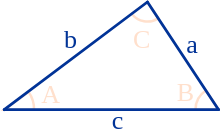
\includegraphics[width=4cm]{./public/images/sss}
    \caption[SSS]{side, side, side}
\end{figure}

The \textbf{Law of Cosines} can be used to find angles.